\subsection{Skalierungsstrategien}
\label{sec:scale}

Die in den vorangegangenen Abschnitten beschriebenen Techniken zum Aufbau von Recommender-Systemen entfalten vor allem bei einer möglichst großen Datenbasis ihren Nutzen. Der Umfang der zu diesem Zweck erhobenen Daten steigt schnell in Größen die nichtmehr sinnvoll von einzelnen Systemen verarbeitet werden können.  Um  diesem Problem zu begegnen, beschreibt dieser Abschnitt mögliche Lösungsstrategien zur Speicherung, Verteilung und Verarbeitung von Daten auf einer großen Zahl von Rechnern. \todo[color=green]{ggf. Langford09 Parallelisierungsstrategien dazu}

\subsubsection{Skalierung der Datenhaltung}

Die Architektur eines Dateisystems dass den Ansprüchen großer verteilter Systeme genügt wird in \citep{ghemawat03} beschrieben. Das darin entworfene \acf{GFS} orientiert sich dabei an den Erfahrungen aus dem praktischen Anwendungen und stellt folgende Kernannahmen:

\begin{itemize}
\item Das Gesamtsystem wird aus vielen handelsüblichen und damit günstigen Komponenten aufgebaut. Da Ausfälle einzelner Komponenten keine Ausnahme darstellen, müssen diese automatisch erkannt und behoben bzw. tolerant ausgeglichen werden.
\item Die typische Größe der verwalteten Dateien bewegt sich über dem 100 MB Bereich, mehrere Gigabyte große Dateien sind eher der Regelfall und sollten für das System kein Problem darstellen. Aus diesem Grund sollte das Dateisystem für die Verwaltung von großen Dateien optimiert werden. 
\item Dateien werden vorwiegend durch lange, kontinuierliche Lesezugriffe (Streaming) genutzt welche große zusammenhängende Bereiche der Dateien nutzen. Kleine wahlfreie Zugriffe auf Teile der Dateien können von den Anwendungen oft zu Leseoperationen von größeren Bereichen zusammengefasst werden.
\item Schreibzugriffe erfolgen ebenfalls vorwiegend auf große zusammenhängenden Bereichen. Bereits geschriebene Bereiche werden zudem selten geändert, d.h. neue Daten werden in der Regel an das Ende einer Datei angehängt.
\item Einzelne Dateien werden oft von mehreren Quellen gleichzeitig beschrieben. Deshalb muss das Dateisystem die Synchronisation dieser Quellen mit möglichst wenig Zusatzaufwand ermöglichen.
\item Um möglichst effizient große Datenmengen ``am Stück'' verarbeiten zu können, hat die Ausnutzung der Schreib/Lesebandbreite hohe Priorität. Der Latenz einzelner Operationen wird geringeres Gewicht beigemessen.
\end{itemize}

Diese Annahmen begründen zentrale Eigenschaften des Systems. Ein \acs{GFS}-Cluster wird aus einem \textit{Master}- und vielen \textit{Chunkservern} aufgebaut. Jede Datei wird in Blöcke (engl. Chunks) mit einer festen Größe von 64 MB aufgeteilt. Die Speicherung der Blöcke erfolgt im lokalen Dateisystem der \textit{Chunkserver}. Zur Gewährleistung der Verfügbarkeit wird jeder Block auf mehrere \textit{Chunkserver} repliziert. Die Verwaltung der zum Betrieb notwendigen Metadaten wird von \textit{Masterserver} übernommen. D.h. jeder \textit{Chunkserver} kennt nur die von ihm verwalteten Blöcke, welche durch ein eindeutiges 64 Bit \textit{Handle} identifiziert werden. Die Zuordnung der Blöcke zu Dateien, die Verwaltung der Dateistrukturen, die Rechteverwaltung und die Verteilung der Blöcke zwischen den \textit{Chunkservern} obliegt dem \textit{Masterserver}.

Um zu verhindern das Flaschenhälse entstehen, werden Daten weitestgehend ohne den \textit{Masterserver} gelesen und geschrieben. Einzig um den Speicherort eines Blockes zu finden oder um strukturelle Operationen durchzuführen (Erzeugen, Umbenennen, Löschen, ... ) wird er von den Anwendungen benötigt. Alle weiteren Operationen geschehen direkt zwischen den \textit{Chunkservern} und der Anwendung. Die Größe der Blöcke minimiert zudem den Kommunikationsaufwand zwischen Anwendung und \textit{Masterserver}, da mit jeder Anfrage ein sehr großer Datenbereich abgedeckt werden kann. Um dennoch konsistente Ergebnisse beim Schreiben neuer Daten zu erhalten wird zwischen der Anwendung und den \textit{Chunkservern} ein fest definiertes Kommunikationsprotokoll verfolgt welches sicherstellt, dass Änderungen tatsächlich bei allen Servern gleich geschrieben wurden bevor die entsprechende Operation erfolgreich abgeschlossen wird (vgl. \citep[Kap. 3]{ghemawat03}).

Alle Operationen die vom \textit{Masterserver} ausgeführt werden, werden zudem in einem \textit{Operation Log} gesichert. Fällt er aus, kann er leicht mit Hilfe der gesicherten Logs  durch einen neuen \textit{Masterserver} ersetzt werden. Wie bei den Blockoperationen, werden auch Schreiboperationen in das Log nur dann als erfolgreich abgeschlossen wenn sie auch auf allen vorhandenen Realisationen erfolgreich ausgeführt wurden. Das ``Wissen'' der \textit{Chunkserver} über die auf ihnen gespeicherten Blöcke minimiert zudem die im \textit{Operation Log} gehaltenen Informationen.

Die Integrität der Daten wird von den \textit{Chunkservern} sichergestellt. Innerhalb der 64 MB Blöcke werden Prüfsummen für jeden 64 KB Abschnitt geschrieben. Stellt der \textit{Chunkserver} beim Lesen fest, dass die Daten eines Blockes beschädigt sind, wird vom \textit{Master} veranlasst, dass der Block von einem anderen \textit{Chunkserver} ausgeliefert wird und das er zu einem weiteren repliziert wird. Ist dies geschehen, wird der beschädigte Block entfernt.

Wie in  \citep{ghemawat03}  gezeigt wird, kann ein so aufgebautes System auf der Basis von handelsüblichen Hardware effizient betrieben werden, falls die zuvor beschriebenen Annahmen für die damit betriebenen Anwendungen zutreffen.  \citep{ghemawat03}

\subsubsection{Horizontalen Fragmentierung}

Will man große Datenmengen innerhalb eines Datenspeichers halten ohne an die Grenzen einzelner Speicherknoten zu stoßen, ist die \textit{horizontale Fragmentierung} (engl. \textit{Sharding}) eine weitere mögliche Strategie. Zur Verarbeitung einer Anfrage sind hierfür zwei Knotentypen bzw. Servertypen notwendig. Die \textit{Backend-Knoten} halten jeweils einen Teil der Daten und verarbeiten alle Anfragen dafür. Die \textit{Frontend-Knoten} bilden die Schnittstelle zu den Applikationen. Sie verteilen die Anfragen an die richtigen Backend-Knoten und fassen Anfrageergebnisse verschiedener Backend-Knoten zusammen. In der Regel werden die Daten möglich gleichmäßig mit Hilfe eines, über einen Hashing-Algorithmus generierten, Schlüssels auf die Backend-Knoten verteilt. \citep{Michael07}
\begin{figure}[H]
  \centering
    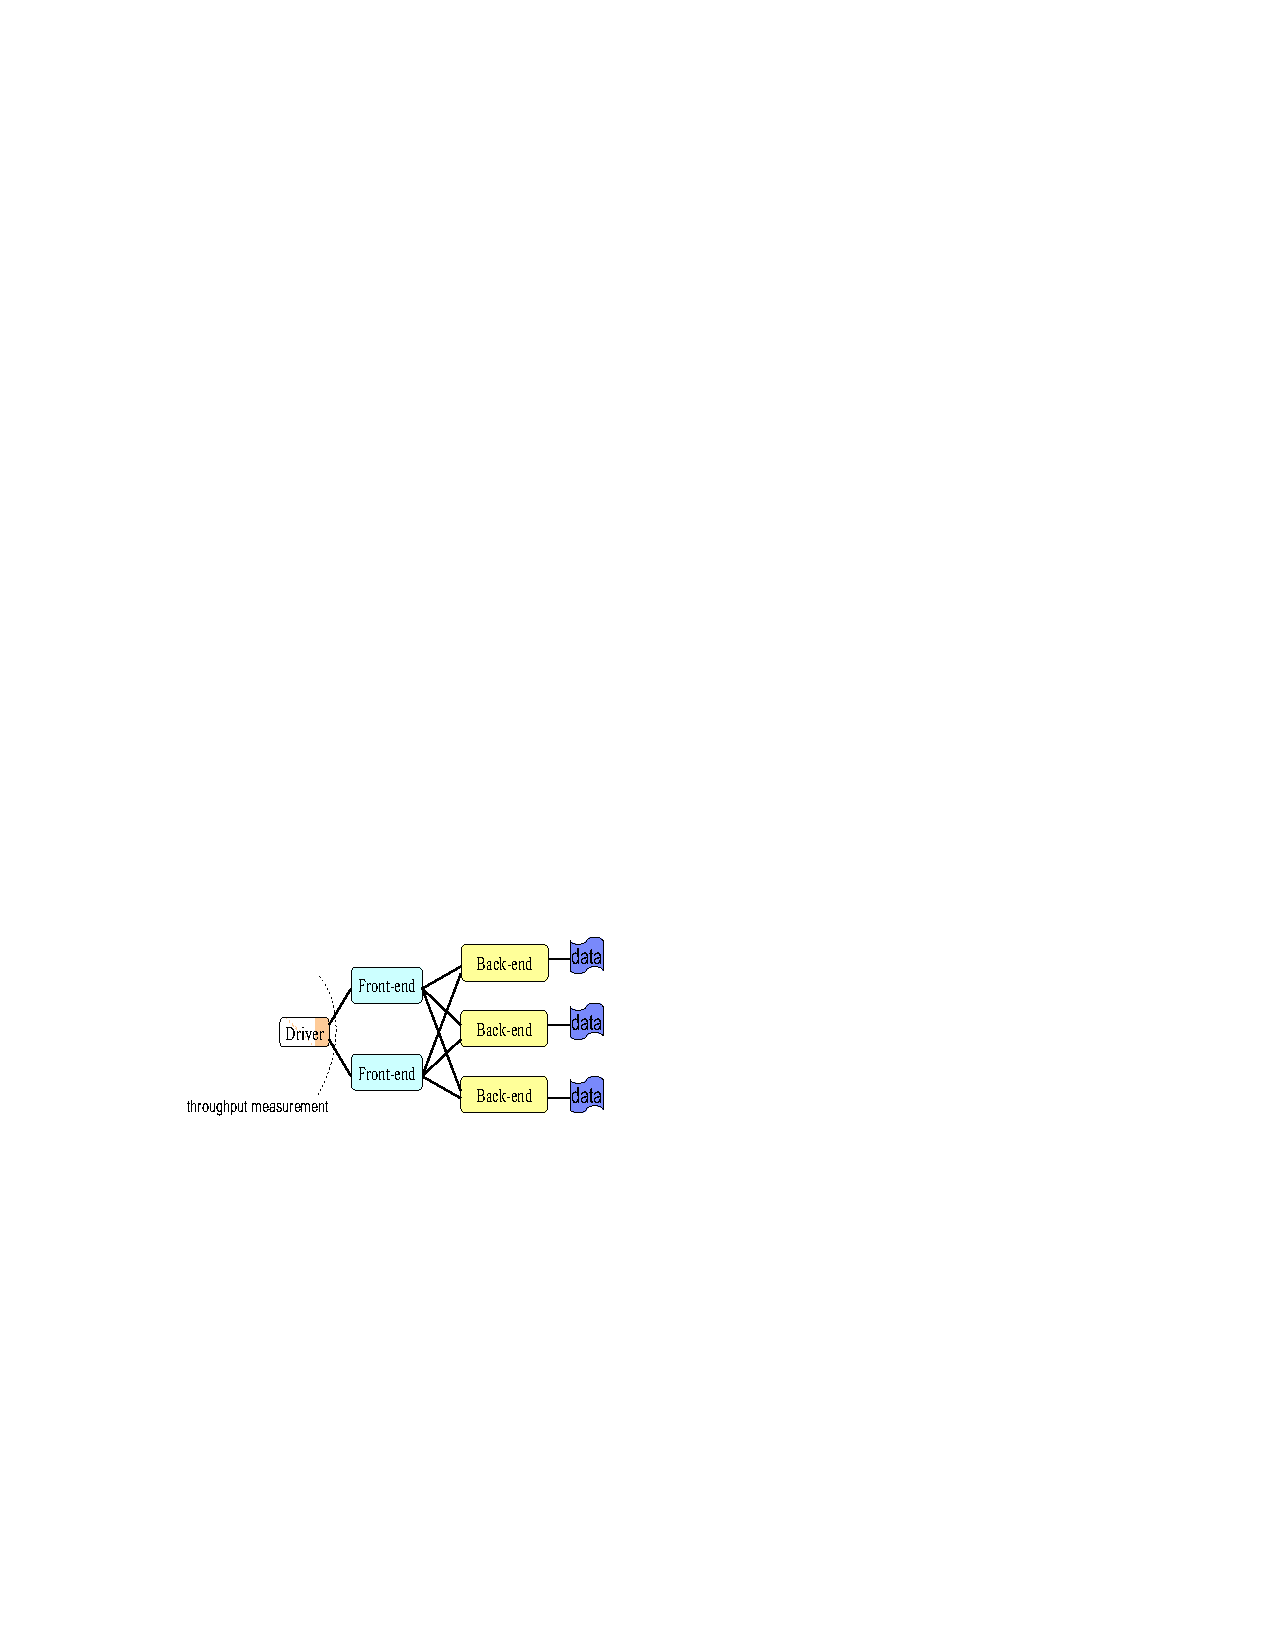
\includegraphics[width=0.5\textwidth]{Abbildungen/sharding}
    \caption[Horizonale Fragmentierung]{\footnotesize Abfragestruktur horizontal fragmentierter Systeme {\footnotemark} }
    \label{fig:sharding}
\end{figure}
\footnotetext{Quelle: \citep{Michael07}}

Der Nachteil einer derartigen Verteilung ist, dass Transaktionen um atomare Operationen zu gewährleisten erheblichen Zusatzaufwand nach sich ziehen. In Bereichen wo diese nicht notwendig sind, etwa bei der Verwaltung von Suchindexen, kann horizontale Fragmentierung allerdings zu signifikanten Leistungssteigerungen führen. \citep{Michael07}

\subsubsection{MapReduce basierte Algorithmen}

Liegen die Daten in einem verteilten System vor, muss auch die Verarbeitung über viele Systeme verteilt werden. Mit \textit{MapReduce} wird in \citep{mapred04} ein dafür geeignetes Programmier-Paradigma vorgestellt. 

 Die Eingabe- und Ausgabedaten der Verarbeitung bestehen aus einfach strukturierten Parameter-Wert Paaren (engl. Key-Value Pairs), welche in den drei festen Phasen \textit{Map}, \textit{Shuffle} und \textit{Reduce} verarbeitet werden. In der \textit{Map}-Phase wird jeder Datensatz einzeln und unabhängig von anderen durch die Anwendung verarbeitet. Die Unabhängigkeit ermöglicht es, diesen Schritt auf viele parallele Prozesse zu verteilen und die Verarbeitung sehr ``nah'' bei den Daten --- also über das gesamte verteilte System hinweg --- durchzuführen. Die Ergebnisse der Verarbeitung --- wiederum ein Parameter-Wert Paar --- werden in der darauffolgenden  \textit{Shuffle}-Phase entsprechend der Parameter sortiert. In der abschließenden  \textit{Reduce}-Phase werden alle zu einem Parameter gehörenden Werte gemeinsam verarbeitet. Die Verarbeitung der Gruppen erfolgt wieder unabhängig von anderen, so dass auch dieser Schritt auf viele parallele Prozesse und Rechenknoten verteilt werden kann. \citep{mapred04} \todo[color=green]{Ggf. MapRed. Beispiel einfügen.}

Trotz des sehr einfachen Verarbeitungsschemas ist es möglich, komplexe Algorithmen mit \textit{MapReduce} auszuführen. In \citep{mapred06} werden für zahlreiche Algorithmen des maschinellen Lernens die dafür notwendigen Umformungen beschrieben und analysiert. Grundlage der Umformungen ist das in \citep{Kearns98} beschriebene \textit{Statistical Query Model}. Dieses ermöglicht es, statistische Konzepte für Testdatensätze zu untersuchen und aus diesen darin vermutete statistische Verteilungen abzuleiten. Auf dieser Basis beschreibt \citep{mapred06} wie spezielle Algorithmen umgeformt werden können, um diese durch die Bildung von Teil-Approximationen und nachgelagerte Zusammenfassung in eine verteilbare \textit{MapReduce} Form zu überführen. Die so umgeformten Algorithmen skalieren nahezu linear mit der Anzahl der verfügbaren Rechenknoten bzw. Prozessorkernen. Dass diese Umformungen auch für die in Abschnitt \ref{sec:filtermethods}  beschriebenen Algorithmen des kollaborativen Lernens möglich sind, wird in \citep{jiang11} gezeigt. \citep{mapred06} \todo{BSP}

\subsubsection{Skalierung der Filtermodelle}

Die zuvor beschriebenen allgemeineren Methoden zur Verteilung und Verarbeitung großer Datenmengen sind im Zusammenhang mit Filtermodellen (vgl. Abschnitt \ref{sec:filtermethods}) vor allem im Bereich der Vorverarbeitung bzw. des Trainings relevant. 

Geht man davon aus, dass zur Verarbeitung eines einzelnen Bewertungseintrages 48 Byte im Speicher belegt werden, so stößt man bei ``üblichen'' 16 GB Hauptspeicher nach ca. 300 Millionen Einträgen an die Grenzen eines einzelnen Knotens. Auch wenn effizientere Speichernutzung --- etwa durch die Reduktion von Objektreferenzen --- den Speicherbedarf pro Eintrag auf 28 Byte senkt (vgl. \citep{mia}), ist es dennoch ratsam erheblich früher verteilte Algorithmen zu nutzen. Wie \citep{mapred06} und \cite{jiang11} zeigen, profitieren Systeme mit mehreren Prozessorkernen ebenfalls signifikant von der Parallelisierung durch \textit{MapReduce}.

Da die Laufzeit aller in Abschnitt \ref{sec:filtermethods} beschriebenen Modelle von der Anzahl der Nutzer und Elemente anhängig ist, machen es große Datenmengen zudem sehr schwer Empfehlungen ``online'' zu berechnen. Die Reduktion der verarbeiteten Informationen (zB. durch Cluster-Mechanismen) ist eine möglicher Ausweg. Da dadurch allerdings auch Informationen verloren gehen, sind die resultierenden Ergebnisse auch ungenauer. Einen möglichen Kompromiss zur Erzeugung von schnellen und präzisen Ergebnisse beschreibt \citep{linden03}. Alle rechenaufwendigen Verarbeitungsschritte, wie zum Beispiel die Berechnung von Element- oder Nutzerähnlichkeiten (vgl. Abschnitt \ref{sec:neighborhoods}), werden in eine Vorverarbeitungsphase verschoben und nur die eigentliche Generierung der Empfehlungen geschieht ``online''. Als Ergebnis der Vorverarbeitung erhält man entsprechend eine Matrix die Nutzer zu allen anderen Nutzern bzw. Elemente zu allen anderen Elementen korreliert. Der Rechenaufwand zur Generierung der Empfehlungen ist dann nur noch abhängig von der Anzahl der vom Nutzer gekauften bzw. bewerteten Elemente. Ein wichtiger Nachteil ist, dass neue Daten erst verspätet in das abgeleitete Filtermodell einfließen können, dies kann abhängig von der ``Stabilität'' der Datenbasis, zum Beispiel wenn Elemente nur kurze Zeit ``verfügbar'' sind (vgl. \citep{Cornelis20074906}), ein Ausschlussfaktor für Offline-Berechnungen sein. \citep{linden03}


%
% - Recommendation Datenmodelle die "schnell" sind
% - die meisten arbeiten mit "In-Memory" Datenmodellen (mit Optimierte Speicherung für die Ausführung)
%        - Wo sind die Grenzen (user,item anzahl ?)
%        - Lösungen: Precomputing similarities? 
%  - Lösungen: Cluster-based recommendation
%- Wann macht distributed recommendation sinn
%  - Ist Offline recommendation dafür ein Use-Case (Calculation recommendations and send via mail)?
%  - Das lernen der Datenmodelle muss auch skalieren
%- Hadopp etc...
%
%\citep{Vidal:2005:PDR:2137725.2137737}
%\citep{Toscher:2008:INA:1722149.1722153}
%http://techblog.netflix.com/2012/06/scalable-logging-and-tracking.html
%\subsubsection{Online- / Offline-Recommendation}
% BigTable http://labs.google.com/papers/bigtable-osdi06.pdf 